\chapter{Technical Background} \label{ch:technical_background}

In this chapter, we provide an overview of the theory, which is crucial for understanding the person re-ID approaches that will be described in the following chapters. 

We start with the description of the terms Deep learning, Artificial neuron, and describe a general artificial neural network. Later, we continue with the convolutional neural networks, recurrent neural networks, long-short term neural networks and convLSTM neural networks. We will also explain the edge extraction and joints detection methods, the we use in the data pre-processing phase in our experiments.

\section{Deep learning}\label{tb:deep_learning}
Deep learning is part of machine learning, which is based on Artificial Neural Networks \cite{DLWiki}. The idea of the Artificial Neural Networks (ANN) first emerged in the 1940s after McCulloch and Pitts introduced simplified neurons in 1943 \cite{NN_introduction}. The ANNs are inspired by the biological neural networks that are present in the brain. The reason why the ANNs are gaining much attention in the recent years is that they have been shown to outperform previous state-of-the-art techniques in several tasks and together with the increasing amount of available data in fields like computer vision, they are believed to have a great potential in the future.

\subsection{Artificial Neuron}\label{tb:ann}
The Artificial Neuron is the elementary unit of every ANN. It represents a function $f$, which process an input $\textbf{x}=[x_1, x_2, ..., x_n]$ such that
\begin{equation}
    f(\textbf{x)}=\varphi(F(\textbf{x}))= \varphi(\sum_{i=1}^{n}w_ix_i + b).
\end{equation}
In the above equation, the function $\varphi$ is a so called activation function, which decides, whether a neuron should be activated and what is its relevance. The main purpose of the activation function is to introduce non-linearity into the output of a neuron. This is important as most real-world problems are not linear and the neural networks need to be able to learn these non-linear representations. The scalars $w_1,...,w_n$ are learnable weights and scalar $b$ is a learnable bias.

The neurons in a neural network are connected by connections and the learnable weights represent the significance of this connections. Each input to a neuron consists of outputs of previous neurons that have a connection with the current neuron. Figure \ref{fig:neuron} shows a diagram of a single neuron.

\begin{figure}[h!]
    \centering
    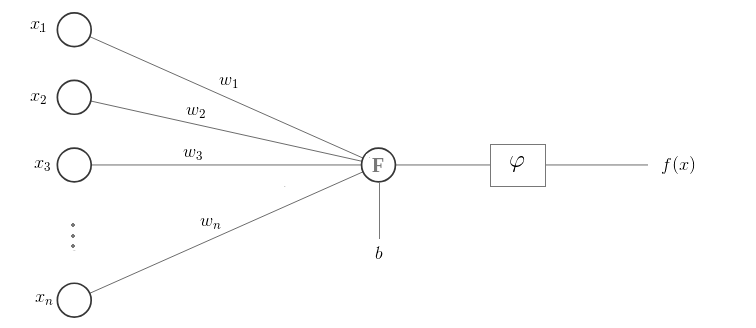
\includegraphics[scale=0.4]{figures/neuron.png}
    \caption{Neuron} 
    \label{fig:neuron}
\end{figure}

\subsection{General ANNs}\label{tb:ann}
Every ANN consists of an input layer, one or more hidden layers, and an output layer. Every layer contains multiple neurons, and they have connections to neurons from adjacent layers. In case all neurons from one layer are connected to all neurons from the previous layer, we talk about a dense (or fully connected) layer. An example of a neural network with two hidden layers can be seen in Figure \ref{fig:simple_ann}.

\begin{figure}[h!]
    \centering
    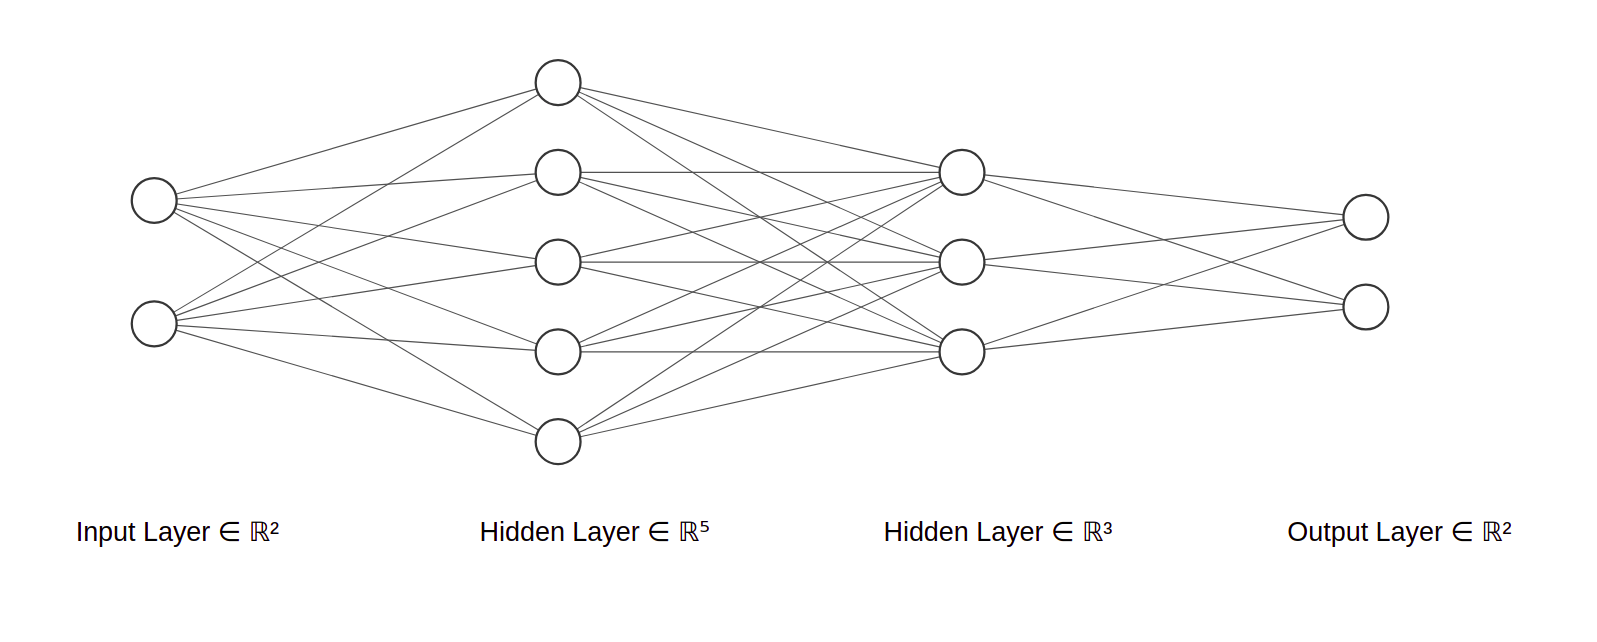
\includegraphics[scale=0.2]{figures/simple_nn.png}
    \caption{Artificial Neural Network diagram} 
    \label{fig:simple_ann}
\end{figure}

\subsection{Convolutional Neural Networks}\label{tb:cnn}
Convolutional neural networks (CNNs) are a particular type of ANNs, that were originally designed for the usage in image processing applications. The characteristics of CNNs is the usage of convolution in at least one of its layers. 

The reason why CNNs are so widely used in computer vision problems is that even small-sized images contain a tremendous amount of information. A grey-scale $620\times480$ image contains 297 600 pixels. Assuming that every pixel intensity of this image is an input to a fully-connected network, each neuron of this network requires 297 600 weights. Hence, the number of free parameters in the network becomes extremely large as the image size increases. This leads to overfitting and slow performance. In CNNs, the total number of free parameters is reduced using the convolutional layers.

Another reason for the usage of CNNs is its translation invariance. In many pattern detection tasks, the same pattern can be found in different places in the image, and it would be inefficient to train neurons to recognize the same pattern on different positions independently.

A CNN usually consists of three types of layers: convolutional layers, pooling layers, and fully connected layers.

\subsubsection{Convolutional Layers}

In the convolutional layers, every neuron represents a convolution of a filter (called kernel) and a small patch in the image. The neurons are applied along the width and height dimensions of the image. The kernels have the same depth as the images, but smaller width and height. The output width and height of each layer depend on the kernel size, number of strides (number of pixels that the kernel is shifted between each computation) and the number of zero-padding pixels around the input image. 

The main trick of the convolutional layers is the fact that the trainable weights (filters) are shared among a number of neurons in one layer. Hence, the number of free parameters in the convolutional layer is significantly lower than in a fully connected layer. The output from a convolution of the input with one filter (all neurons sharing the same weights) is called a feature map. Each filter in one layer generates one feature map, and together they make up the output depth. Every entry in the feature map can be interpreted as the output of one neuron. 

Figure \ref{fig:ConvNN} displays a mapping of a convolutionar layer. 
Every patch from the input on the left hand side (one example is highlighted by the red block) is convolved with all filters of the layer. The convolutions of all patches from the input with one filter produce one feature map (one of them is highlighted by the red plane on the right). The whole output consists of all feature maps, where the number of feature maps corresponds to the number of filters in this layer.

Every feature map detects some feature in the input. For example, in image processing, one feature map can detect horizontal edges, another one vertical edges, etc.

\begin{figure}[h!]
    \centering
    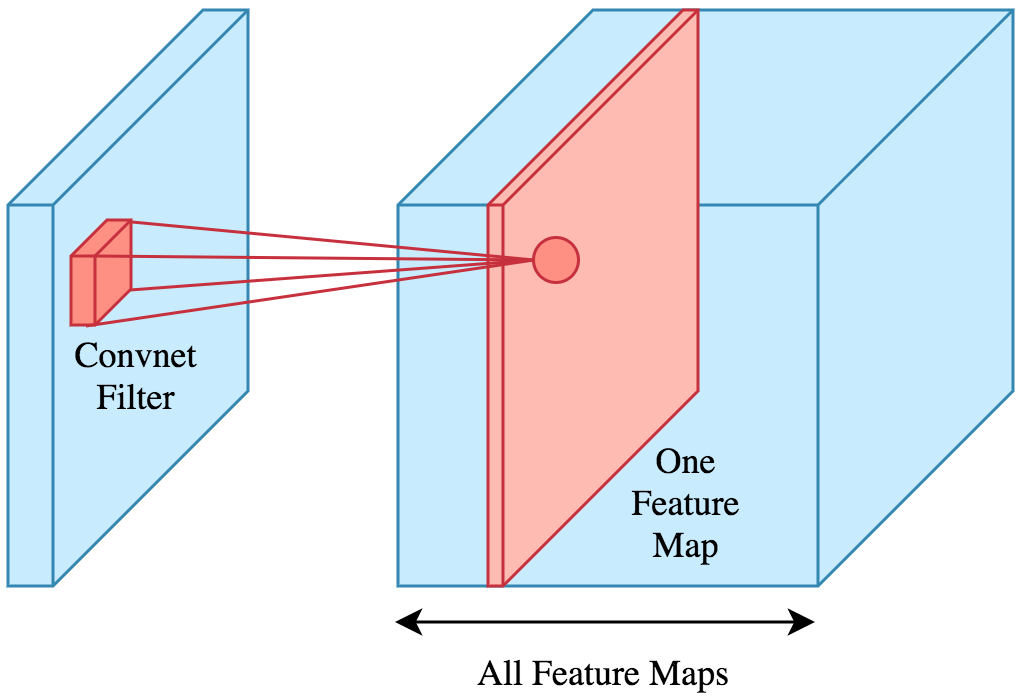
\includegraphics[scale=0.2]{figures/convNN.png}
    \caption{Convolutional layer \cite{ConvNN_layer_img}}
    \label{fig:ConvNN}
\end{figure}

\subsubsection{Pooling Layers}
The Pooling Layers progressively reduce the size of the data passed throw them, and hence, they reduce the number of parameters of the network. There are several non-linear functions which can be used for pooling. The most common one is max pooling, where the input is partitioned into rectangles from which the max value is selected. 

\begin{figure}[h!]
    \centering
    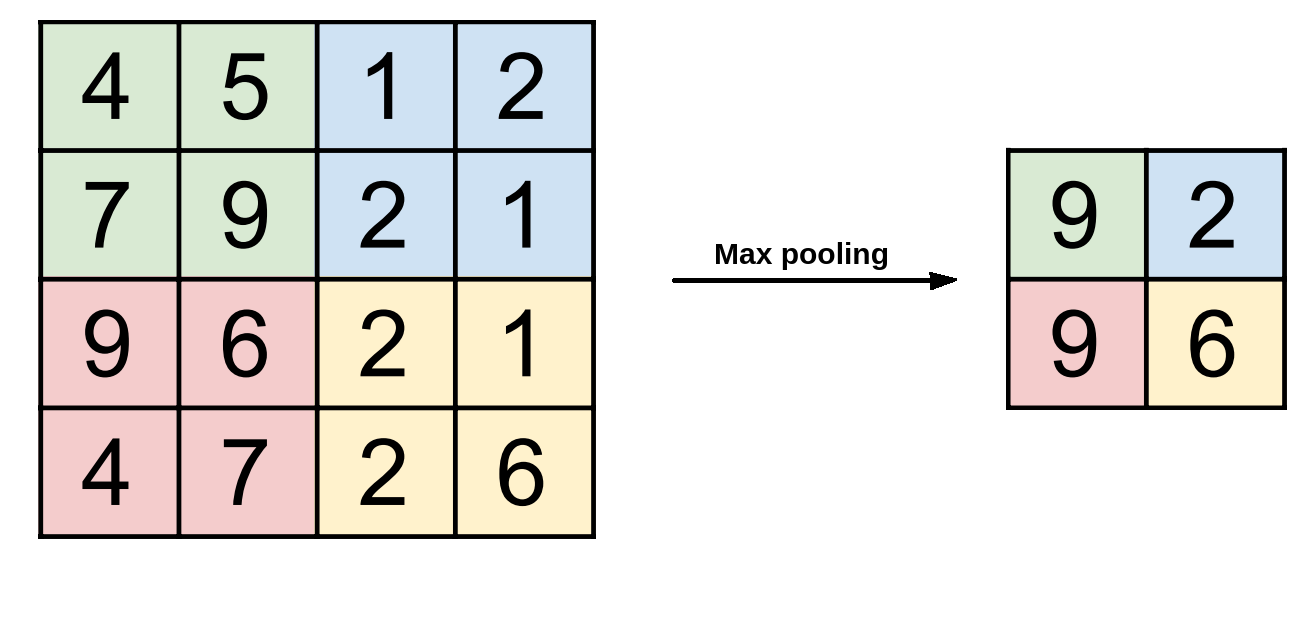
\includegraphics[scale=0.2]{figures/max_pooling.png}
    \caption{Max pooling}
    \label{fig:maxPooling}
\end{figure}

\subsubsection{Fully Connected Layers}
In the CNNs, the Fully Connected Layers are usually present at the end of the network. They are fully connected to all activations in the previous layers and perform the high-level reasoning of the network such as classification based on the features extracted by the preceding layers etc.

\begin{figure}[h!]
    \centering
    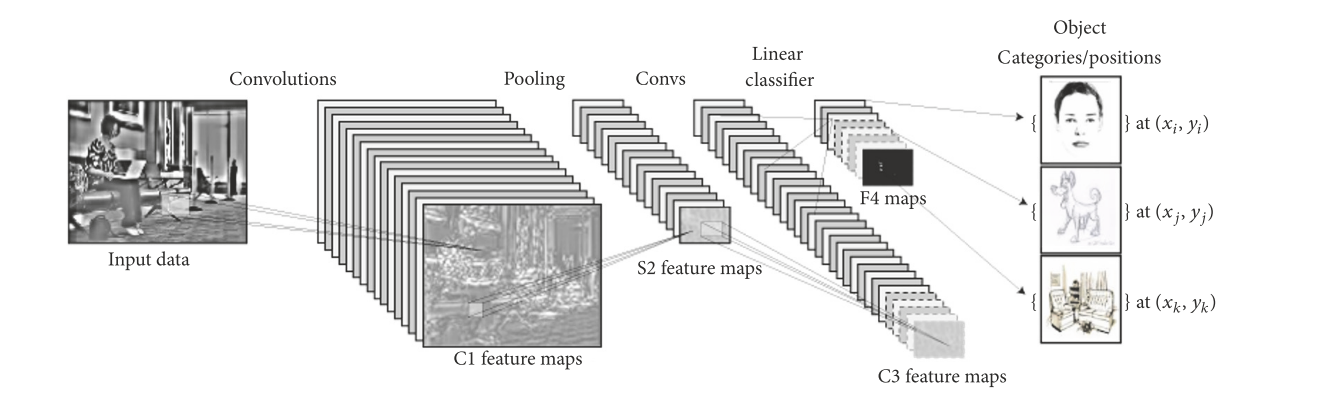
\includegraphics[scale=0.3]{figures/CNN_example.png}
    \caption{CNN architecture example \cite{DL_for_computer_Vision}}
    \label{fig:DL}
\end{figure}

\subsection{Recurrent Neural Networks}\label{tb:rnn}
The traditional feed-forward neural networks are a powerful tool with many applications. However, one of their shortcomings is that when applied on sequential data, they fail to capture the sequential structure as they are not able to reason about the output based on the previously seen outputs. This is where the Recurrent Neural Networks (RNNs) come into play. They are networks with loops in them, allowing the output to be influenced not only by the weights that are learned during the training process but also by a state vector representing the context based on previously seen inputs and outputs.

The schema of a recurrent neural network is illustrated in Figure \ref{fig:RNN}. Here, a chunk of a neural network, A, receives the input $x_t$ and produces the output $h_t$. The loop allows information to be passed from one step of the network to the next one. We can also interpret the RNN as a chain of multiple identical network models, each passing a message to the following one (see Figure \ref{fig:RNN_unrolled}).
\begin{figure}[h!]
    \centering
    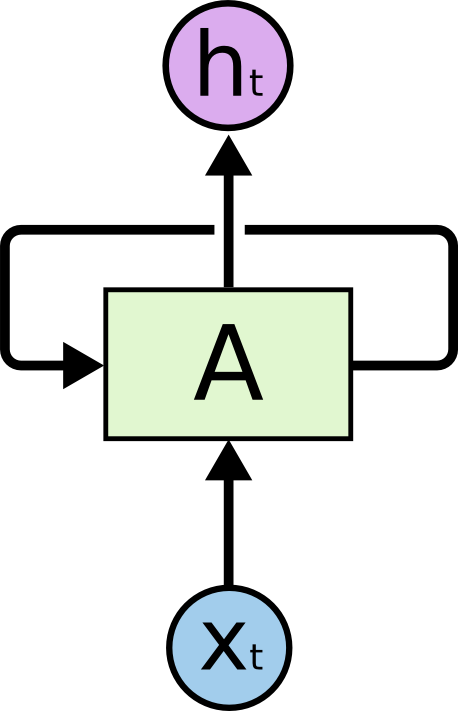
\includegraphics[scale=0.3]{figures/RNN-rolled.png}
    \caption{Recurrent neural network \cite{LSTM_blog}}
    \label{fig:RNN}
\end{figure}

\begin{figure}[h!]
    \centering
    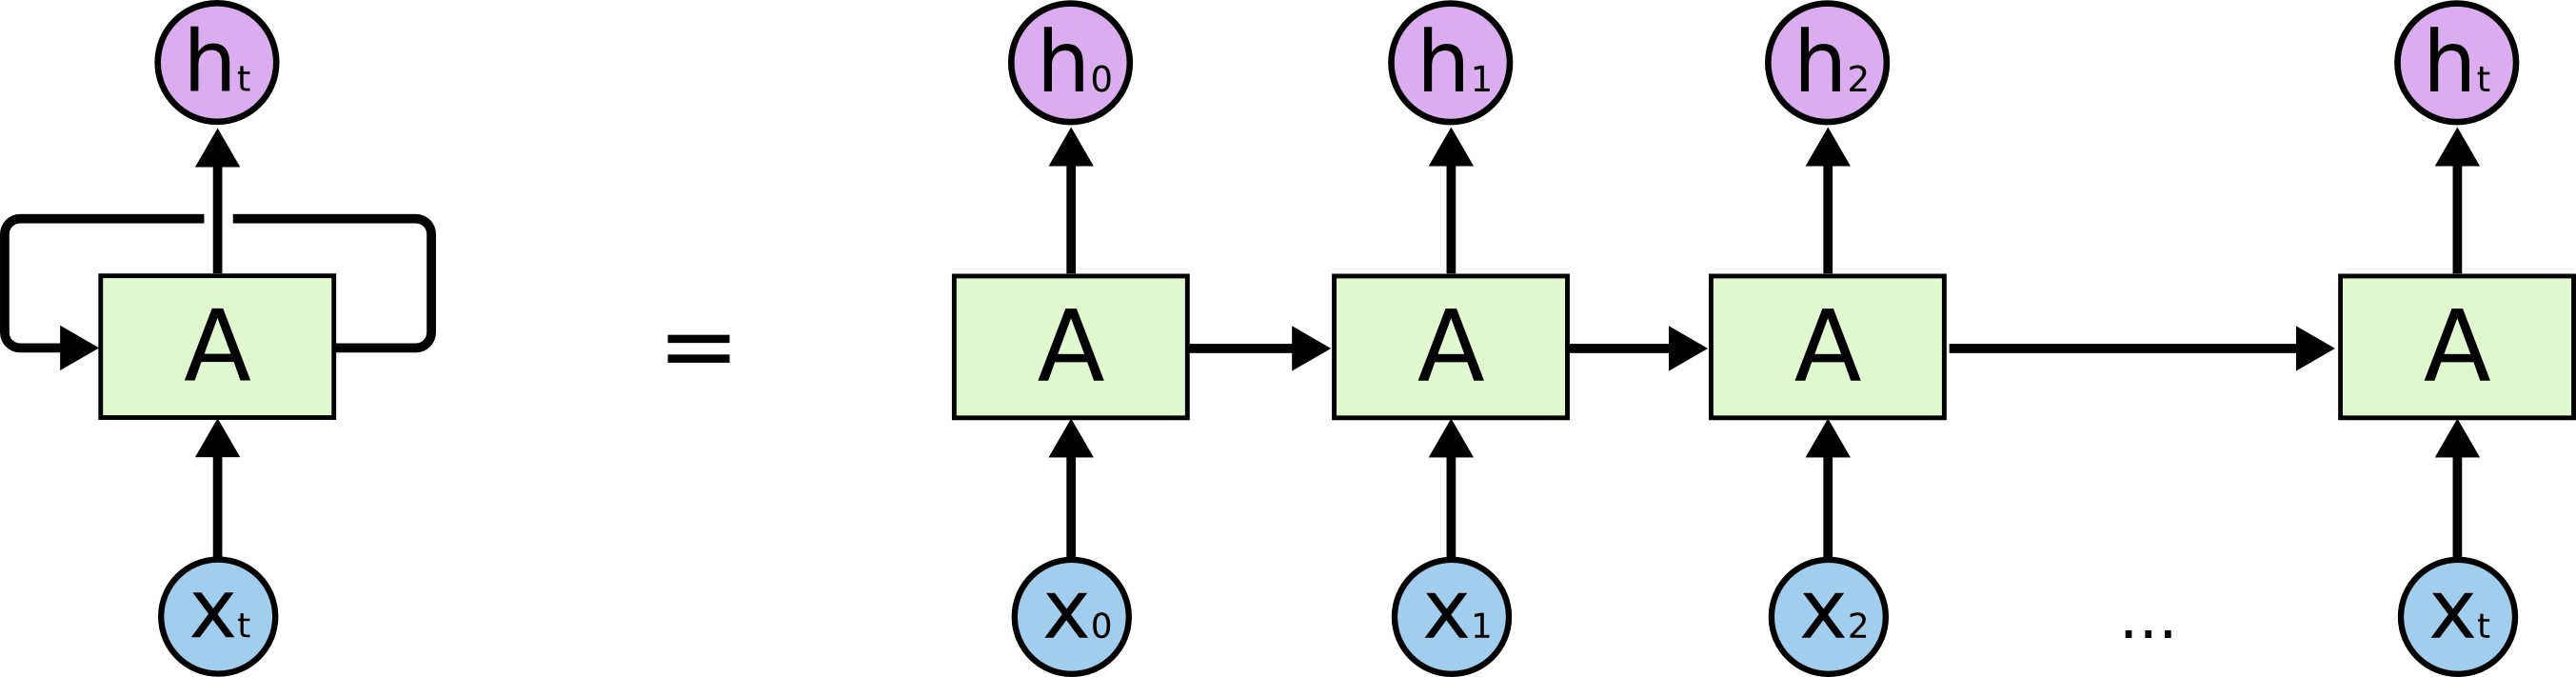
\includegraphics[scale=0.3]{figures/RNN-unrolled.png}
    \caption{Unrolled recurrent neural network \cite{LSTM_blog}}
    \label{fig:RNN_unrolled}
\end{figure}


\subsubsection{The problem of Long-Term Dependencies}

In some cases, it is enough for the network to only remember the last few outputs from a sequence for good reasoning about the newly seen input. However, there are cases where the network needs to look far in the history to be able to classify the output for a given input correctly. In the case of the standard RNNs, the repeating modules have a very simple structure. Usually, they consist of one $tanh$ layer (see Figure \ref{fig:simple_rnn}). In theory, despite their simple structure, RNNs are perfectly able to learn this so-called Long-Term Dependencies. However, in practice, they are not performing well in such situations (see \cite{RNN_long_term} for more information). To overcome this issue, in 1997, Long Short-Term Memory Neural Networks were introduced \cite{LSTM_paper}.


\begin{figure}[h!]
    \centering
    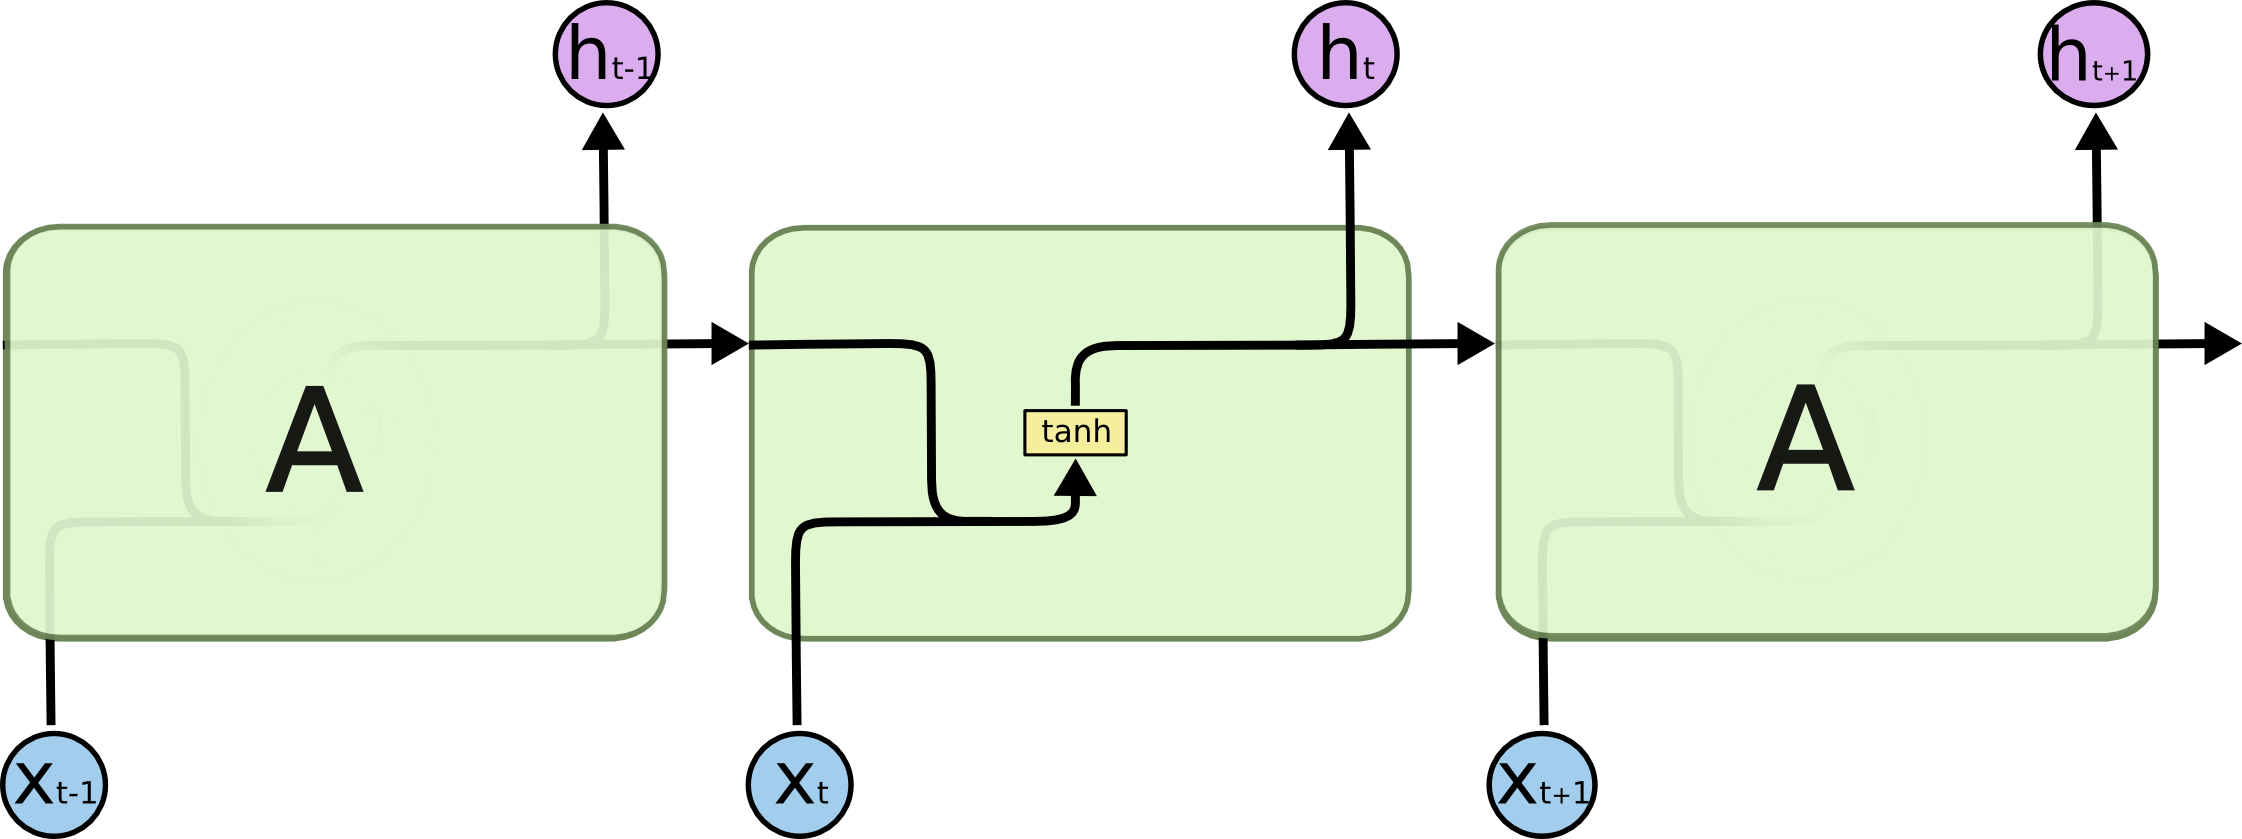
\includegraphics[scale=0.45]{figures/LSTM3-SimpleRNN.png}
    \caption{Repeating module in standard RNNs \cite{LSTM_blog}}
    \label{fig:simple_rnn}
\end{figure}


\subsection{Long Short-Term Memory Neural Networks}\label{tb:lstm}
The Long Short-Term Memory Neural Networks (LTSMs) are a special type of RNNs, which are designed to avoid the long-term dependency problem. Unlike the standard RNNs, LSTMs are able to remember information for long time periods. 


The key difference between the standard RNNs and LSTMs is the structure of the repeating network modules. Instead of having one single neural network layer, the schema of the LSTM repeating module is more complicated (see Figure \ref{fig:lstm_modes_schema}). 


\begin{figure}[h!]
    \centering
    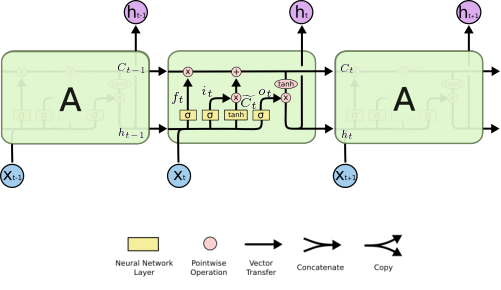
\includegraphics[scale=0.7]{figures/LSTM3-chain.png}
    \caption{Repeating module in standard LSTMs \cite{LSTM_blog}}
    \label{fig:lstm_modes_schema}
\end{figure}


It consists of two parts. The first part is the cell state (the horizontal line passing throw the pointwise addition and pointwise multiplication nodes), which can be thought of as a transporter running down the whole chain of the network models. 

The second part is composed of three so called gates and one $tanh$ layer. The gaits consist of a sigmoid layer and a pointwise multiplication operation and output a number between zero and one, which specifies how much of the component should be remembered. The $tanh$ layer, on the other hand, creates new candidate values, which can be to some extent (depending on the gates) added to the cell state.

The formulation of the LSTM module can be summarized by following equations.

\begin{align}
    f_t &=\sigma(W_{xf}\cdot x_t + W_{hf}\cdot h_{t-1} +b_f)\\
    i_t &=\sigma(W_{xi} \cdot x_t + W_{hi} \cdot h_{t-1} +b_i)\\
    \widetilde{C}_t&=tanh(W_{xC}\cdot x_t + W_{hC} \cdot h_{t-1} +b_C)\\
    C_t&=f_t\circ C_{t-1}+i_t\circ \widetilde{C_t}\\
    o_t&=\sigma(W_{xo} \cdot x_t + W_{ho} \cdot h_{t-1} +b_o)\\
    h_t&=o_t\circ tanh(C_t)
\end{align}
where $\circ$ represents a pointwise multiplication, $\cdot$ a scalar multiplication and $+$ represents a vector addition.

For detail information about the LSTMs, see \cite{LSTM_blog}. 


\subsection{ConvLSTM}\label{tb:convLstm}
We have already explained the convolutional neural networks, which are networks, that are able to learn the spacial dependencies in images, and LSTM networks, that cover the temporal dependencies. However, one might be interested in covering both the special and the temporal dimension (e.g., when processing video sequences). For this case, the Convolutiona LSTMs (convLSTMs) were designed. 

The convLSTMs follow the same structure as the LSTMs, but instead of a matrix multiplication, they use convolution operation inside of the LSTM module. Hence, the input and output data of the convLSTM are 3 dimensional vectors, unlike in the standard LSTM module where the input and output data are one-dimensional. This way, convLSTMs are able to capture the underlying spatial features. 

The formulation of the convLSTM module can be summarized by equations (3.8) throw (3.13). 

\begin{align}
    f_t &=\sigma(W_{xf}* x_t + W_{hf}* h_{t-1} +b_f)\\
    i_t &=\sigma(W_{xi} * x_t + W_{hi} * h_{t-1} +b_i)\\
    \widetilde{C}_t&=tanh(W_{xC}* x_t + W_{hC} * h_{t-1} +b_C)\\
    C_t&=f_t\circ C_{t-1}+i_t\circ \widetilde{C_t}\\
    o_t&=\sigma(W_{xo} * x_t + W_{ho} * h_{t-1} +b_o)\\
    h_t&=o_t\circ tanh(C_t)
\end{align}
where $*$ represents a convolution operation.

For more information about the convLSTMs, see \cite{convLSTM}.

\section{Edge detection}\label{tb:edge_detection}
In the edge detection problem, the task is to find edges and object boundaries in raw images. This problem is of a great importance to a variety of computer vision areas, and hence, a great number of approaches to edge detection have been developed, ranging from early developed method using the Sobel operator \cite{sobel} or Canny detector \cite{canny} to recently developed methods based on convolutional neural networks such as DeepEdge \cite{deepedge} or CSCNN \cite{cscnn}. In this thesis, we use the Holistically-Nested Edge Detection library (HED) available at \cite{xie15hed}, which provides an image-to-image method transforming the raw image into image of the objects boundaries. The method is build upon a deep learning model that leverages fully convolutional neural networks and deeply-supervised nets \cite{deeply_supervised_nets}, adopting a slightly modified VGGNet architecture \cite{vgg}. An example of the HED image transformation can be seen in Figure \ref{fig:hed}. For more information about the HED library, see \cite{xie15hed}.

\begin{figure}[h!]
    \centering
    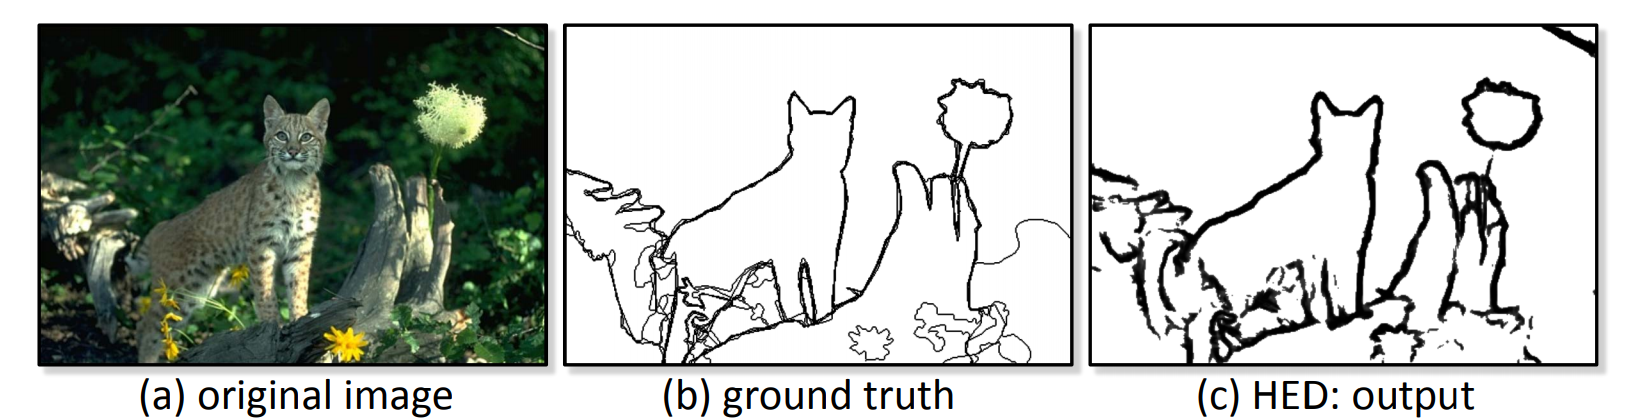
\includegraphics[scale=0.22]{figures/HED.png}
    \caption{HED edge detection example, \cite{xie15hed}}
    \label{fig:hed}
\end{figure}

\section{Skeleton extraction}\label{tb:joints_location}
The task of skeleton extraction (also known as pose estimation) consists in finding the locations of joints of people in a picture or a video and connecting the right ones so that the result forms skeletons of the people. For this purpose, we use in this thesis the Openpifpaf library available at \cite{openpifpaf}.

This library is based on the work by Sven Kreiss at al. \cite{openPifPaf_paper}. It provides a bottom-up method for multi-person 2D human pose estimation. 

The whole method is based on a ResNet \cite{resnet} network with two head networks: PIF (Part Intensity Field), which localizes the body parts, and PAF (Part Association Field) used to associate body parts with each other so that they form full human poses. The whole model is displayed in Figure \ref{fig:pifpaf}. The input is an image of size $(H, W)$ with three color channels. The neural network based encoder produces PIF and PAF fields. The decoder is then applied to convert the PIF and PAF fields into pose estimates containing 17 joints each. Each joint is represented by an $x$ and $y$ coordinate and a confidence score.

For more information, see \cite{openPifPaf_paper}.

\begin{figure}[h!]
    \centering
    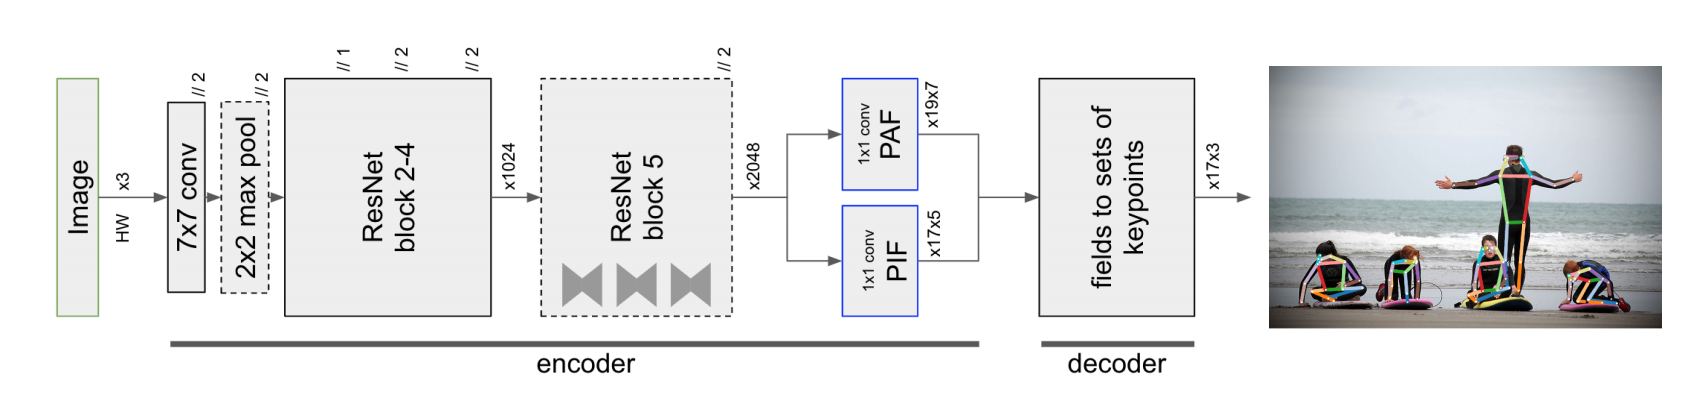
\includegraphics[scale=0.22]{figures/PifPafModel.png}
    \caption{Openpifpaf model \cite{openPifPaf_paper}}
    \label{fig:pifpaf}
\end{figure}

